\documentclass[10pt]{article}
\usepackage{icmlko}

\icmlmeta{IP 파운데이션 월드모델}{284}{열한 번째 방}{시장 팝업을 도메인으로 열었다 --- 우연보다 낫고 아무도 안 해쳤는데, 판 수를 어제와 못 견주게 됐다}

\begin{document}

\twocolumn[
\icmlheader

\begin{abstract}
노트 283이 ``붙이지 말고 따로 열라''로 끝났다. 전제 셋을 확인하고 열었다 ---
\textbf{시간}(\texttt{period\_from} 이 개최일), \textbf{겹침}(내부와 브랜드 ·
기간이 모두 겹치는 진짜 중복 둘을 뺐다. 미래엔 디지털초코 · 블룸타이드,
\emph{자사 프로젝트가 기사가 된 것}), \textbf{라벨}(A · B 만 써도 학습 47행이라
청력 문턱 22 위). 결과는 \textbf{205행 · 학습 101 · 유보 104 · 판 몫 3.9\%}
이고, 도메인 배선은 공유 축 다섯에 태웠다(\texttt{venue\_prominence} $\gets$
\texttt{ip\_history.prior\_count}, \texttt{goods\_scale} $\gets$
\texttt{multi\_store} $\ldots$). 판정은 둘로 갈라 했다. \textbf{①} 새 도메인은
$\rho{=}{+}0.1970$ 이고 치환 귀무 $-$0.0029 $\pm$ 0.0988 대비
\textbf{$z{=}{+}2.02$, $p{=}0.045$} --- 우연보다 낫지만 아슬아슬하다.
\textbf{②} 기존 아홉은 \textbf{진짜 0개}(t 문턱 2.77, 노트 282)이고 순
$-$0.0033 --- 아홉 중 여덟이 음수라 자리바꿈의 무늬는 있지만 하나도 유의하지
않다. \textbf{그런데 판 수가 0.4857 $\to$ 0.4713 이다.} 이건 낮은 $\rho$
도메인을 가중 평균에 더한 \textbf{기계적} 효과이지 나빠진 게 아니다 ---
\textbf{두 수를 견주면 안 된다.} 노트 274의 병이 축이 아니라 \emph{도메인}
수준에서 반복된 것이고, 아침에 만든 지문이 그걸 잡는다(\texttt{ebb429357995}
$\to$ \texttt{685c951e8530}, 공통 아홉의 지문은 불변). 마지막으로 왜 $\rho$ 가
낮은지 갈랐다 --- \textbf{시장팝업은 활성 축이 23 중 넷}이고 나머지 열은
13$\sim$19다. \textbf{약한 도메인이 아니라 굶은 도메인이다.}
\end{abstract}
]

\section{열기 전에 셋을 확인했다}

노트 283이 시장 레코드 207건에 쓸 신호가 있다는 것과(멀티스토어 $+$0.227 ·
IP 이력 $+$0.217 · \texttt{category} $H{=}29.4$), \textbf{내부 팝업에 붙이면
안 된다}는 것을 같이 보였다 --- 손 축 마스크가 내부 100\% 대 시장 0\% 라
마스크 무늬가 곧 출처 표지이고 출처가 라벨을 3.2배로 가른다.

그 노트가 남긴 확인 셋을 했다.

\begin{center}\small
\begin{tabular}{ll}
\hline
전제 & 결과 \\
\hline
① 시간 마스크 & \texttt{period\_from} 이 개최일이다 \\
② 내부와 겹침 & 브랜드 $+$ 기간이 다 겹치는 것 \textbf{둘} \\
③ 라벨 신뢰 & A 2 · B 88 · C 81 · D 11 · E 23 \\
\hline
\end{tabular}
\end{center}

②의 둘은 \textbf{미래엔 디지털초코}(2025-02-21)와 \textbf{블룸타이드}
(2026-04-10)이고, 둘 다 \emph{우리 프로젝트가 기사가 된 것}이다. 뺐다.
(브랜드 문자열만으로는 21건이 걸리는데 기간까지 겹쳐야 진짜다 --- 나머지
열아홉은 같은 모회사의 다른 행사였다.)

③은 C · D · E 가 절반을 넘지만, \textbf{A · B 만 써도 학습 47행}이라 노트
281의 청력 문턱 22 위다. 지금은 전부 쓰고 정제 게이트는 갈래로 남긴다.

\paragraph{그리고 하나 더} 이 도메인은 \textbf{결과로 선택된 모집단}이다 ---
기사가 된 팝업만 있다. 그래서 \emph{그 안에서의 순위 과제}로만 읽고 전체
팝업으로 일반화하지 않는다. 코드 주석과 도메인 설명에 적어 뒀다.

\section{둘로 갈라서 판정한다}

\begin{figure*}[t]
\centering
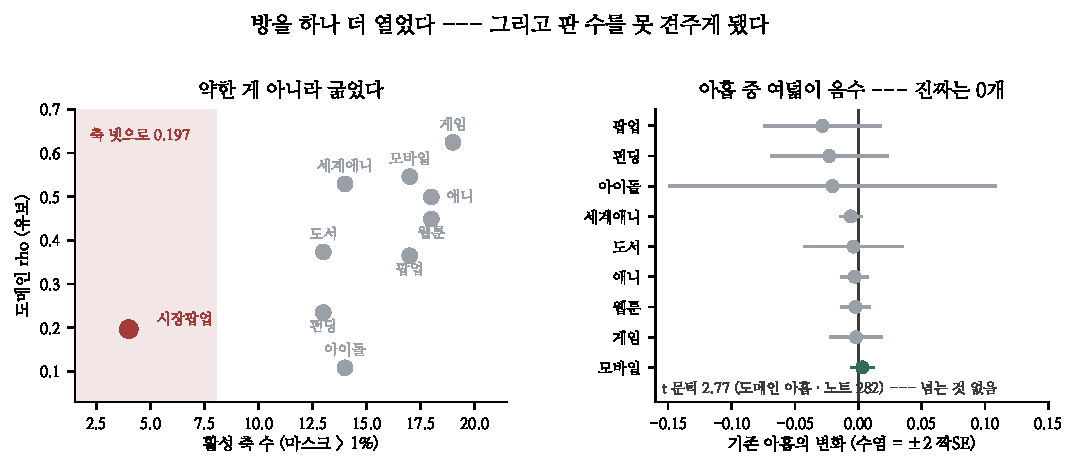
\includegraphics[width=\textwidth]{figs/room.pdf}
\caption{왼쪽 --- 도메인별 활성 축 수와 $\rho$. 오른쪽 --- 새 도메인을 넣었을
때 기존 아홉의 변화(수염은 $\pm$2 짝SE).}
\end{figure*}

도메인을 더하면 판 평균이 \textbf{기계적으로} 바뀐다. 그러니 판 수로 판정하면
안 된다. 둘로 갈랐다.

\paragraph{① 새 도메인이 우연보다 나은가}

\begin{center}\small
\begin{tabular}{lr}
\hline
시장팝업 $\rho$ & \textbf{$+$0.1970} (104행) \\
치환 귀무 & $-$0.0029 $\pm$ 0.0988 \\
& \textbf{$z{=}{+}2.02$ · $p{=}0.045$} \\
\hline
\end{tabular}
\end{center}

\textbf{낫다. 다만 아슬아슬하다.} 이건 계획된 단일 검정이라 노트 282의
다중비교 보정이 안 걸리지만, $p{=}0.045$ 는 한 번 더 봐야 하는 수다.

\paragraph{② 기존 아홉이 흔들리나}

\begin{center}\small
\begin{tabular}{lrrr}
\hline
도메인 & 차 & 짝SE & $t$ \\
\hline
팝업 & $-$0.0282 & 0.0226 & $-$1.25 \\
펀딩 & $-$0.0229 & 0.0227 & $-$1.01 \\
아이돌 & $-$0.0204 & 0.0641 & $-$0.32 \\
세계애니 & $-$0.0058 & 0.0039 & $-$1.48 \\
$\cdots$ & & & \\
모바일 & $+$0.0032 & 0.0041 & $+$0.78 \\
\hline
\multicolumn{4}{l}{순 $-$0.0033 · \textbf{진짜 0개} (t 문턱 2.77)} \\
\hline
\end{tabular}
\end{center}

\textbf{아홉 중 여덟이 음수다} --- 노트 258 · 259가 잰 자리바꿈의 무늬다.
\textbf{그런데 하나도 유의하지 않다.} 노트 282가 고친 문턱(2.77)으로도, 옛
문턱(2.0)으로도 0개다. 제일 큰 것이 팝업 $-$0.0282($t{=}{-}1.25$)인데 팝업은
짝SE 가 0.023 이라 원래 못 재는 자리다(노트 274).

\section{판 수를 못 견주게 됐다}

\textbf{판이 0.4857 $\to$ 0.4713 이다.} 언뜻 크게 나빠 보인다. \textbf{아니다.}
$\rho{=}0.197$ 짜리 도메인을 몫 3.9\% 로 가중 평균에 더하면 평균이 내려간다 ---
\textbf{같은 모형이 더 많은 세상을 덮게 된 것}이지 나빠진 게 아니다.

\begin{quote}\small
어제의 0.4857 은 열 도메인의 판이고 오늘의 0.4713 은 열한 도메인의 판이다.
\textbf{이름이 같고 가리키는 것이 다르다.}
\end{quote}

노트 274$\sim$275가 하루에 세 번 걸린 병이 \emph{축}에서 났는데, 여기서는
\emph{도메인}에서 같은 모양으로 난다. 다행히 아침에 만든 지문이 이걸 잡는다.

\begin{center}\small
\begin{tabular}{lr}
\hline
10 도메인 지문 & \texttt{ebb429357995} \\
11 도메인 지문 & \texttt{685c951e8530} \\
공통 아홉의 지문 & \textbf{전부 불변} \\
\hline
\end{tabular}
\end{center}

\textbf{\texttt{store.comparable} 이 이제 이 두 실행을 ``일부 다름''으로
답한다.} 도메인 수준까지 덮인다는 것을 오늘 확인했다.

\paragraph{그래서 기준선을 다시 놓는다} 앞으로의 판 수는 \textbf{11 도메인
기준 0.4713} 에서 센다. 옛 수와 나란히 적을 때는 도메인 수를 같이 적는다.

\section{왜 0.197 인가 --- 굶었다}

마지막으로 갈랐다. 시장팝업이 낮은 것은 도메인이 나빠서인가?

\begin{center}\small
\begin{tabular}{lrr}
\hline
도메인 & 활성 축 & $\rho$ \\
\hline
게임 & 19 & 0.624 \\
웹툰 · 애니 & 18 & 0.449 · 0.499 \\
팝업 · 모바일 & 17 & 0.365 · 0.546 \\
아이돌 · 세계애니 & 14 & 0.109 · 0.529 \\
도서 · 펀딩 & 13 & 0.374 · 0.235 \\
\textbf{시장팝업} & \textbf{4} & \textbf{0.197} \\
\hline
\end{tabular}
\end{center}

\textbf{활성 축이 23 중 넷이다.} 나머지 열은 13$\sim$19 다. 검색 · 위키 ·
달력 · 태그가 전부 마스크 0 이고 손 축도 \texttt{media\_push} 가 비어 있다.
\textbf{축 넷으로 0.197 을 낸 것이다.}

\textbf{약한 도메인이 아니라 굶은 도메인이다.} 그리고 이 도메인은 브랜드 ·
IP 이름을 갖고 있으니 \textbf{검색 · 위키를 채울 수 있다} --- 다른 도메인이
그걸로 얻은 것이 판 $+$0.148(팝업, 노트 274) 규모였다.

\paragraph{남은 것}
\begin{center}\small
\begin{tabular}{ll}
\hline
갈래 & 왜 \\
\hline
검색 · 위키 채우기 & 축 4 $\to$ 10$+$. 브랜드 이름이 있다 \\
\texttt{category} 전용 축 & $H{=}29.4$ 인데 아직 안 넣었다 \\
정제 게이트 & A · B 만으로 다시 --- 학습 47행 \\
$p{=}0.045$ 재확인 & 씨앗을 갈아 한 번 더 \\
\hline
\end{tabular}
\end{center}

\paragraph{규약} \textbf{도메인을 더하면 판 수의 기준선을 다시 놓는다.}
그리고 \textbf{도메인을 더한 판정은 둘로 갈라서 한다} --- 새 도메인이 우연보다
나은가, 기존이 흔들리나. 가중 평균 하나로 보면 ``좋은 도메인을 더해도 판이
내려가는'' 자리가 생기고, 그건 모형이 아니라 눈금의 성질이다.

\end{document}
